% -*- coding: utf-8 -*-
\RequirePackage{luatex85}
\documentclass[final,xcolor={cmyk,hyperref}]{beamer}
\usepackage[orientation=portrait, size=a0, scale=1.26]{beamerposter}
\usepackage[utf8]{inputenc}
\usepackage{pdfrender}
\usepackage{ifthen}
\usepackage[pdf15,x-1a1]{pdfx}
\FOGRAXXXIX
\usepackage[prefix=]{xcolor-material}
\usepackage{baap-2018-poster}
\usepackage{multicol}
\usepackage{tikz}
\renewcommand{\thefigure}{\Alph{figure}}
\setlength{\abovecaptionskip}{0pt}
\setlength{\belowcaptionskip}{0pt}
\newbox\tikzfigurebox%
\tikzset{%
  figure label/.style={circle, font=\large\bfseries, inner sep=0.125in, outer sep=0,
  fill=kau-light-blue,text=White}
}
\newenvironment{tikzfigure}[1][]{%
\expandafter\xdef\csname tikzfigure@label@#1\endcsname{\thefigure}%
\setbox\tikzfigurebox=\hbox\bgroup}
{\egroup\begin{tikzpicture}%
\node (@) [anchor=south, inner sep=0, outer sep=0]{\box\tikzfigurebox};
\node [figure label, anchor=north]
at ([shift=(90:0.25in)]@.north west) {\thefigure};
\setbox0=\vbox{\caption{somecaption}}
\end{tikzpicture}}
\def\tikzfigureref#1{\hskip0.125ex
\tikz[baseline=(@.base)]\node[figure label,
anchor=base, inner sep=0.333ex, font=\small\bfseries]{\csname tikzfigure@label@#1\endcsname};
}
\setbeamertemplate{caption}[numbered]

\setlength{\leftmargini}{1.25em}

\bibliography{bibliography}

\title{Learning to speak in a second language:
does multiple talker production training benefit
production of English vowels by Arabic-speaking children?}

\author[shortname]{%
Wafaa Alshangiti\texorpdfstring{\,\textsuperscript{1} \and}{,}
Bronwen G. Evans\texorpdfstring{\,\textsuperscript{2} \and}{,}
Mark Wibrow\texorpdfstring{\,\textsuperscript{3} \and}{}}

\institute[shortinst]{
\textsuperscript{1}\,English Language Institute, King Abdulaziz University, Jeddah, Saudi Arabia \qquad
\textsuperscript{2}\,Department of Speech, Hearing \& Phonetic Science, University College London, London, UK \qquad
\textsuperscript{3}\,Cloudfind, Bath, UK}

\def\ipa#1{\textcolor{ipa}{\DejaVuSans\scalebox{0.9}{#1}}}
\def\ipabib#1{\DejaVuSans\scalebox{0.9}{#1}}
\def\word#1{\emph{#1}}
\def\CALVin{{\CraftyGirls%
  \textpdfrender{%
    TextRenderingMode=FillStroke,
    LineWidth=4pt
  }{%
    \textcolor{Red500}{C}%
    \textcolor{LightGreen500}{A}%
    \textcolor{LightBlue500}{L}%
    \textcolor{Amber500}{V}%
    \hskip.125ex%
    \textcolor{Purple500}{in}%
  }}}

\def\chisq{\begingroup\DejaVuSans\char"03C7\endgroup\textsuperscript{2}}
\def\textem#1{\emph{#1}}

\newbox\tmptitlebox
\setbeamertemplate{block begin}{%
  \vskip.5ex
  \begin{beamercolorbox}[leftskip=0.5cm,colsep*=.75ex]{block title}%
    \setbox\tmptitlebox=\hbox{\usebeamerfont*{block title}\insertblocktitle}%
    \dp\tmptitlebox=0.5ex\relax%
    \box\tmptitlebox%
  \end{beamercolorbox}%
  {\ifbeamercolorempty[bg]{block body}{}{\nointerlineskip\vskip-0.5pt}}%
  \usebeamerfont{block body}%
  \begin{beamercolorbox}[colsep*=.75ex,sep=.5ex,vmode]{block body}%
    \ifbeamercolorempty[bg]{block body}{\vskip-.25ex}{\vskip-.75ex}\vbox{}%
  }%
  \setbeamertemplate{block end}{%
  \end{beamercolorbox}%
}

\begin{document}

\begin{frame}[t]

\begin{columns}[t]

\begin{column}{0.4\linewidth}
\begin{block}{Introduction}
  \begin{itemize}
    \item \Cabin
  High-variability phonetic training (HV) has been shown to be
  highly effective in improving second-language (L2)
  perception in adults, and may generalize to production
  \cite{bradlow_etal_2008}
    \item
  In contrast, there have been suggestions that children may
  benefit more from low-variability phonetic training (LV),
  particularly with regard to category discrimination and
  production \cite{evans_martin-alverez_2016}
  \item
  Previous work \cite{alshangiti_2015} trained adult Arabic-speaking
  learners of English in their production of SSBE vowels
  using a computer-based training programme CALVin (Computer Assisted Learning for Vowels interface).
 The results were in line with previous work for consonants \cite{hattori_2009}
 in that training appeared to be domain-specific
 \item
 The current study adapts CALVin for children, to investigate the effect of
 HV and LV production training on Arabic-speaking children
  \end{itemize}
\end{block}

\begin{block}{Methods}
\paragraph{Participants}
\begin{itemize}
  \item 46 monolingual Arabic-speaking Saudi children (aged 10 -- 12)
  \item 22 completed 5 sessions of High Variability training (HV)
  \item 24 completed 5 sessions of Low Variability training (LV)
\end{itemize}

\vspace*{0.125in}
\paragraph{Pre-tests}
\begin{itemize}
  \item
  \textbf{Category discrimination (oddity task)}

  15 highly confusable pairs \cite{alshangiti_2015}, covering 18 vowels,
   produced by 4 SSBE speakers
  (2 female, 2 male) in \ipa{/bVt/} or \ipa{/bVd/} contexts
\end{itemize}

\begin{center}
  \begin{tabular}{@{}rr@{-}ll@{\hskip2ex}rr@{-}ll@{\hskip2ex}rr@{-}ll@{}}
    \word{beat}  & \ipa{/i:/}  & \ipa{/ɪ/}  & \word{bit}
    &
    \word{poot}  & \ipa{/u:/} & \ipa{/ʊ/}   & \word{put}
    &
    \word{bot}   & \ipa{/ɒ/}  & \ipa{/ɑ:/}  & \word{bart}
    \\
    \word{bot}   & \ipa{/ɒ/}  & \ipa{/ʌ/}   & \word{but}
    &
    \word{bert}  & \ipa{/ɜ:/} & \ipa{/ɑ:/}  & \word{bart}
    &
    \word{but}   & \ipa{/ʌ/}  & \ipa{/ɑ:/}  & \word{bart}
    \\
    \word{bird}  & \ipa{/ɜ:/} & \ipa{/eə/}  & \word{bared}
    &
    \word{boat}  & \ipa{/əʊ/} &  \ipa{/aʊ/} & \word{bout}
    &
    \word{bait}  & \ipa{/eɪ/} & \ipa{/e/}   & \word{bet}
    \\
    \word{bait}  & \ipa{/eɪ/} & \ipa{/aɪ/}  & \word{bite}
    &
    \word{bite}  & \ipa{/aɪ/} & \ipa{/ɪ/}   & \word{bit}
    &
    \word{bat}   & \ipa{/æ/}  & \ipa{/ʌ/}   & \word{but}
    \\
    \word{beard} & \ipa{/ɪə/} & \ipa{/eə/}  & \word{bared}
    &
    \word{buoyed} & \ipa{/ɔɪ/} & \ipa{/ɔ:/}  & \word{board}
  \end{tabular}
\end{center}
\begin{itemize}
  \item
  \textbf{Imitation task}

  18 vowels in \ipa{/hVd/} context produced by 1 SSBE female speaker
\end{itemize}
\vspace*{-0.5in}
\begin{center}
  \begin{tabular}{ll@{\hskip1.5ex}ll@{\hskip1.5ex}ll@{\hskip1.5ex}ll@{\hskip1.5ex}ll@{\hskip1.5ex}ll}
    \word{heed}   & \ipa{/i:/} &
    \word{hid}    & \ipa{/ɪ/}  &
    \word{head}   & \ipa{/e/}  &
    \word{heard}  & \ipa{/ɜ:/} &
    \word{had}    & \ipa{/æ/}  &
    \word{hud}    & \ipa{/ʌ/}
    \\
    \word{hard}   & \ipa{/ɑ:/} &
    \word{hod}    & \ipa{/ɒ/}  &
    \word{hoard}  & \ipa{/ɔ:/} &
    \word{who'd}  & \ipa{/u:/} &
    \word{hood}   & \ipa{/ʊ/}  &
    \word{haired} & \ipa{/eə/}
    \\
    \word{hoed}   & \ipa{/əʊ/} &
    \word{how'd}  & \ipa{/aʊ/} &
    \word{hayed}  & \ipa{/eɪ/} &
    \word{hide}   & \ipa{/aɪ/} &
    \word{hear}   & \ipa{/ɪə/} &
    \word{hoyed}  & \ipa{/ɔɪ/}
  \end{tabular}
\end{center}

\paragraph{Post-tests}
\multicolsep=0pt
\begin{multicols}{2}
\begin{itemize}
\item Oddity task
\item Picture naming task
\columnbreak
\item Picture identification task
\item Imitation task
\end{itemize}
\end{multicols}
\end{block}

\vspace*{0.125in}
\begin{block}{Training procedure}

\vspace*{0.25in}

\begin{figure}[h]
\begin{center}
  {\fontsize{128pt}{144pt}\CALVin} \\[0.75ex]
  {\Large\BubblegumSans Computer Assisted Learning for Vowels interface}
\end{center}

\vspace*{0.375in}

\begin{tabular}{ccc}
  \large Low variability (\textbf{LV}) &vs& \large High variability (\textbf{HV})
\\[0.125in]
1 speaker + the instructor
&&
4 speakers  + the instructor
\end{tabular}

\vspace*{0.5in}

\def\screenshotwidth{0.24\linewidth}
\begin{columns}
  \begin{column}{\screenshotwidth}
    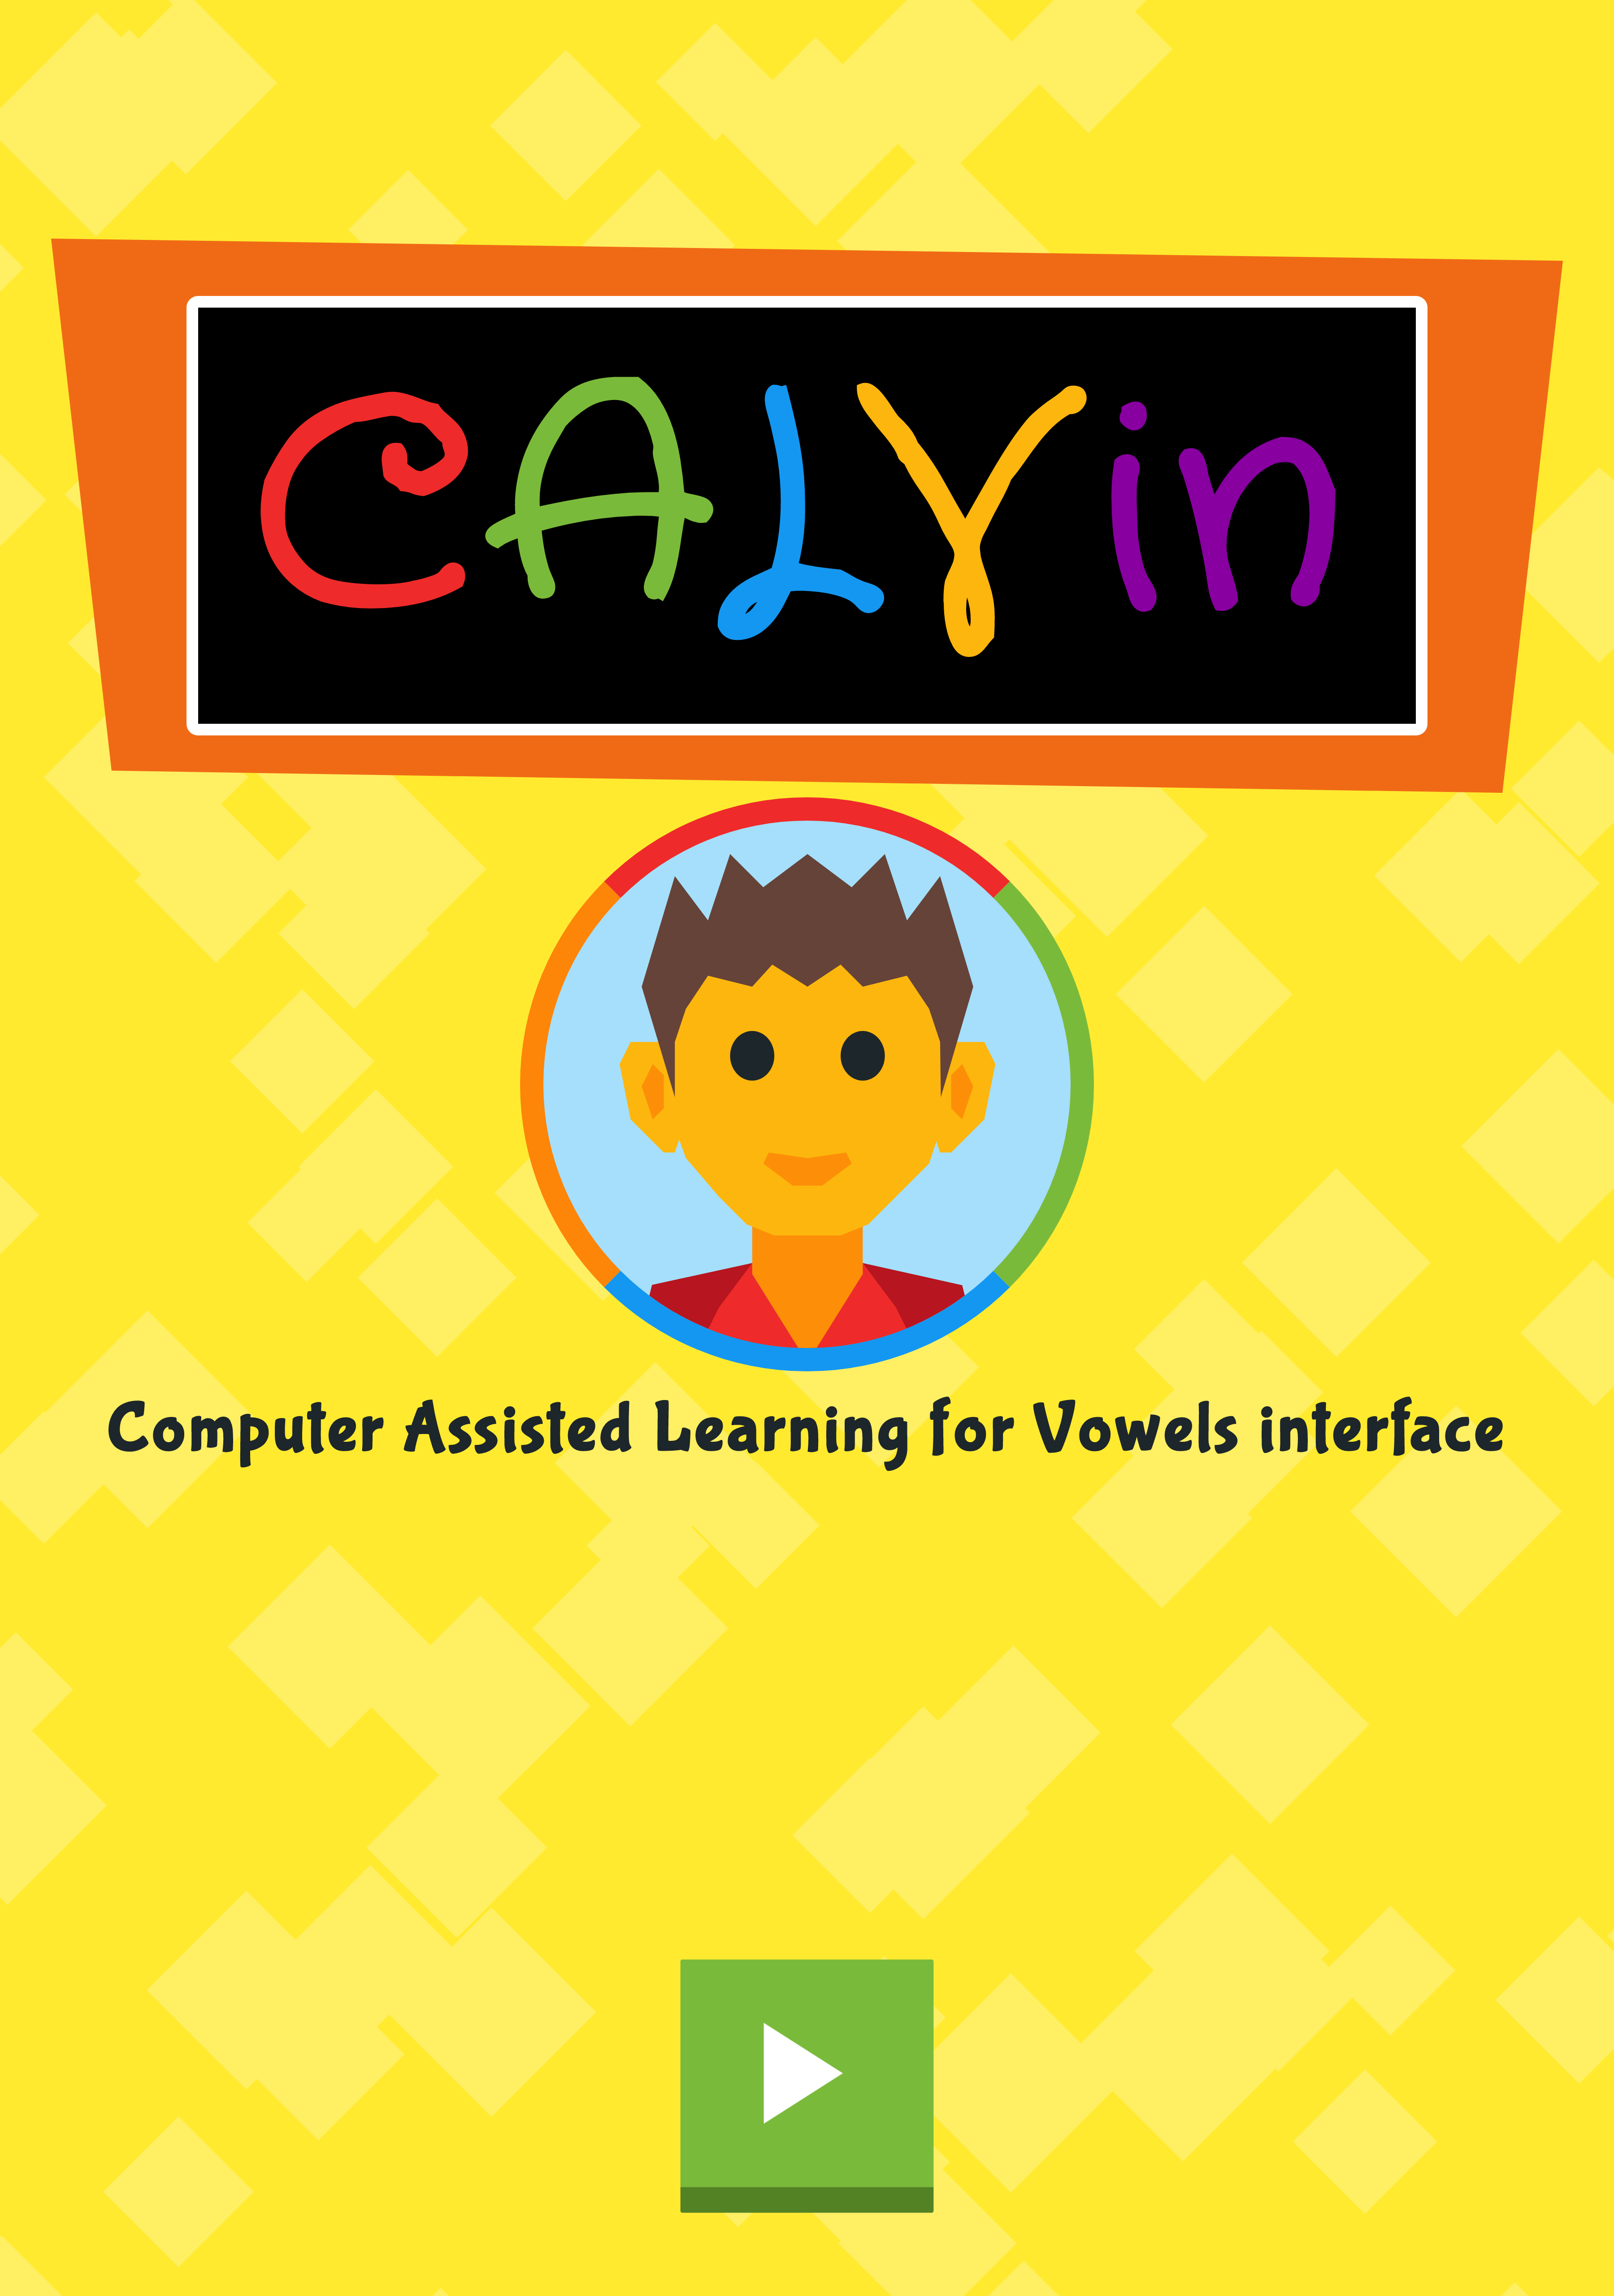
\includegraphics[width=\linewidth]{images/CALVin-screenshots/jpgs/calvin_start}
  \end{column}
  \begin{column}{\screenshotwidth}
    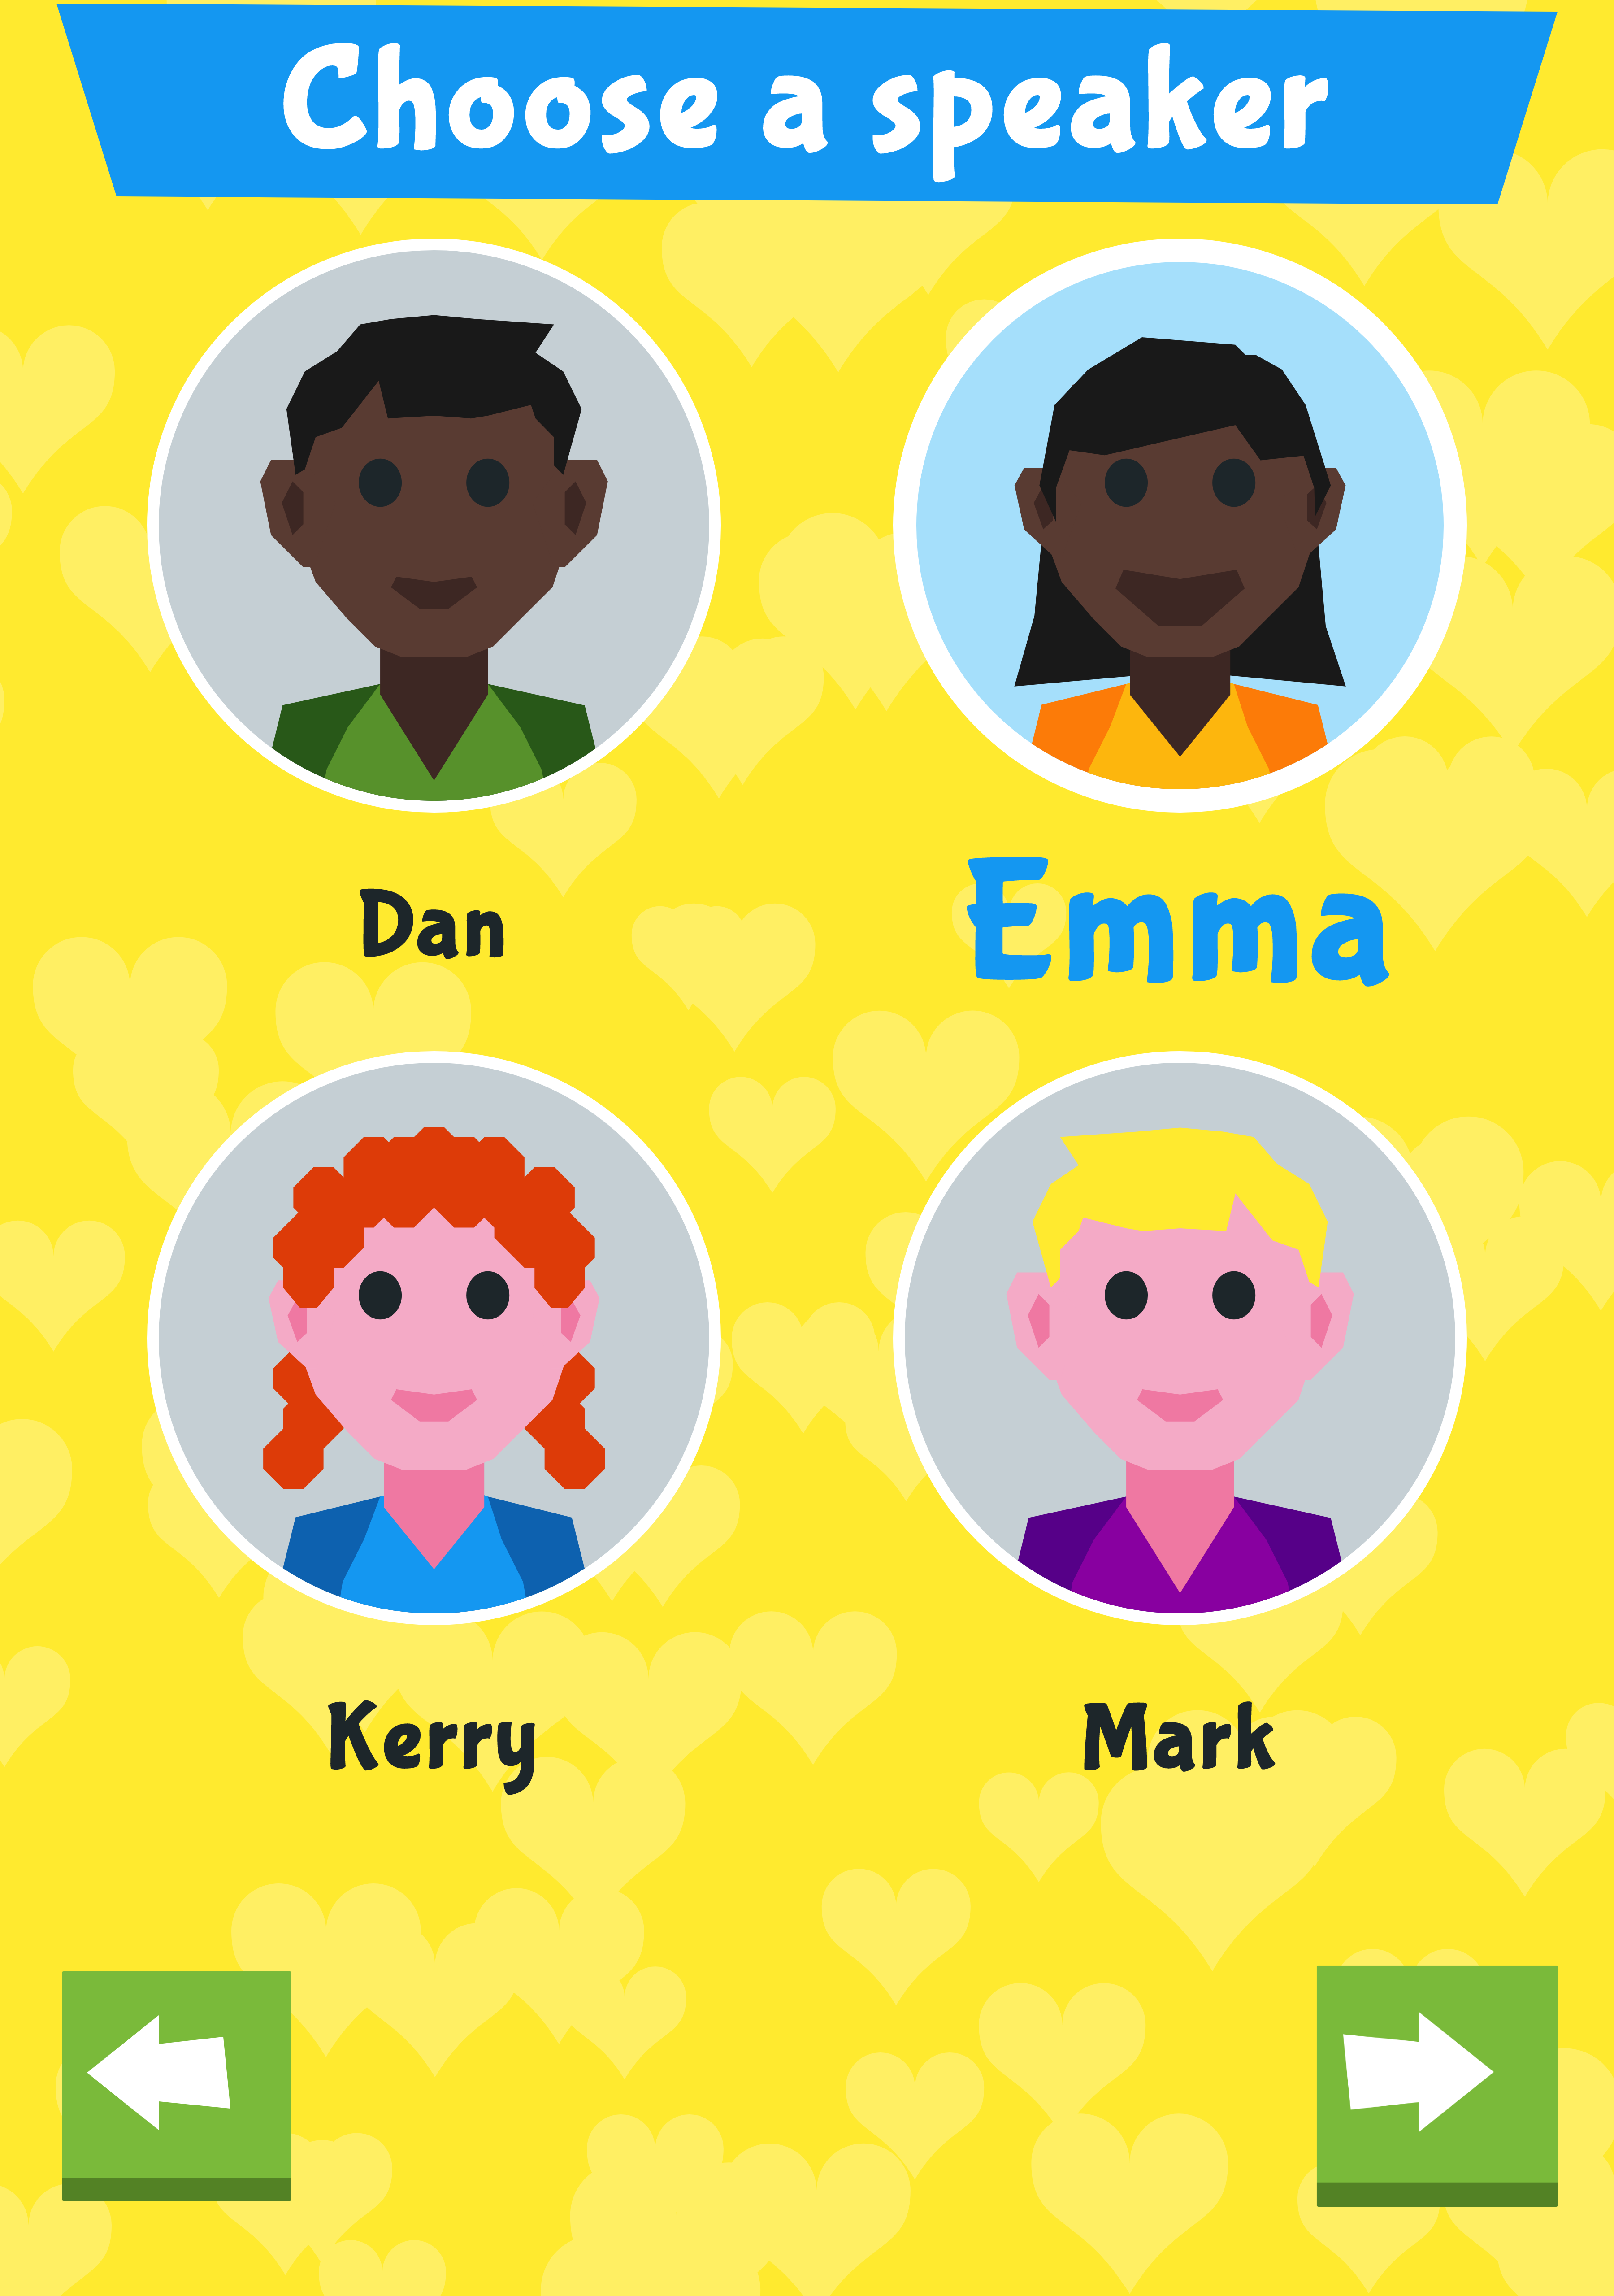
\includegraphics[width=\linewidth]{images/CALVin-screenshots/jpgs/choose_talker}
  \end{column}
  \begin{column}{\screenshotwidth}
    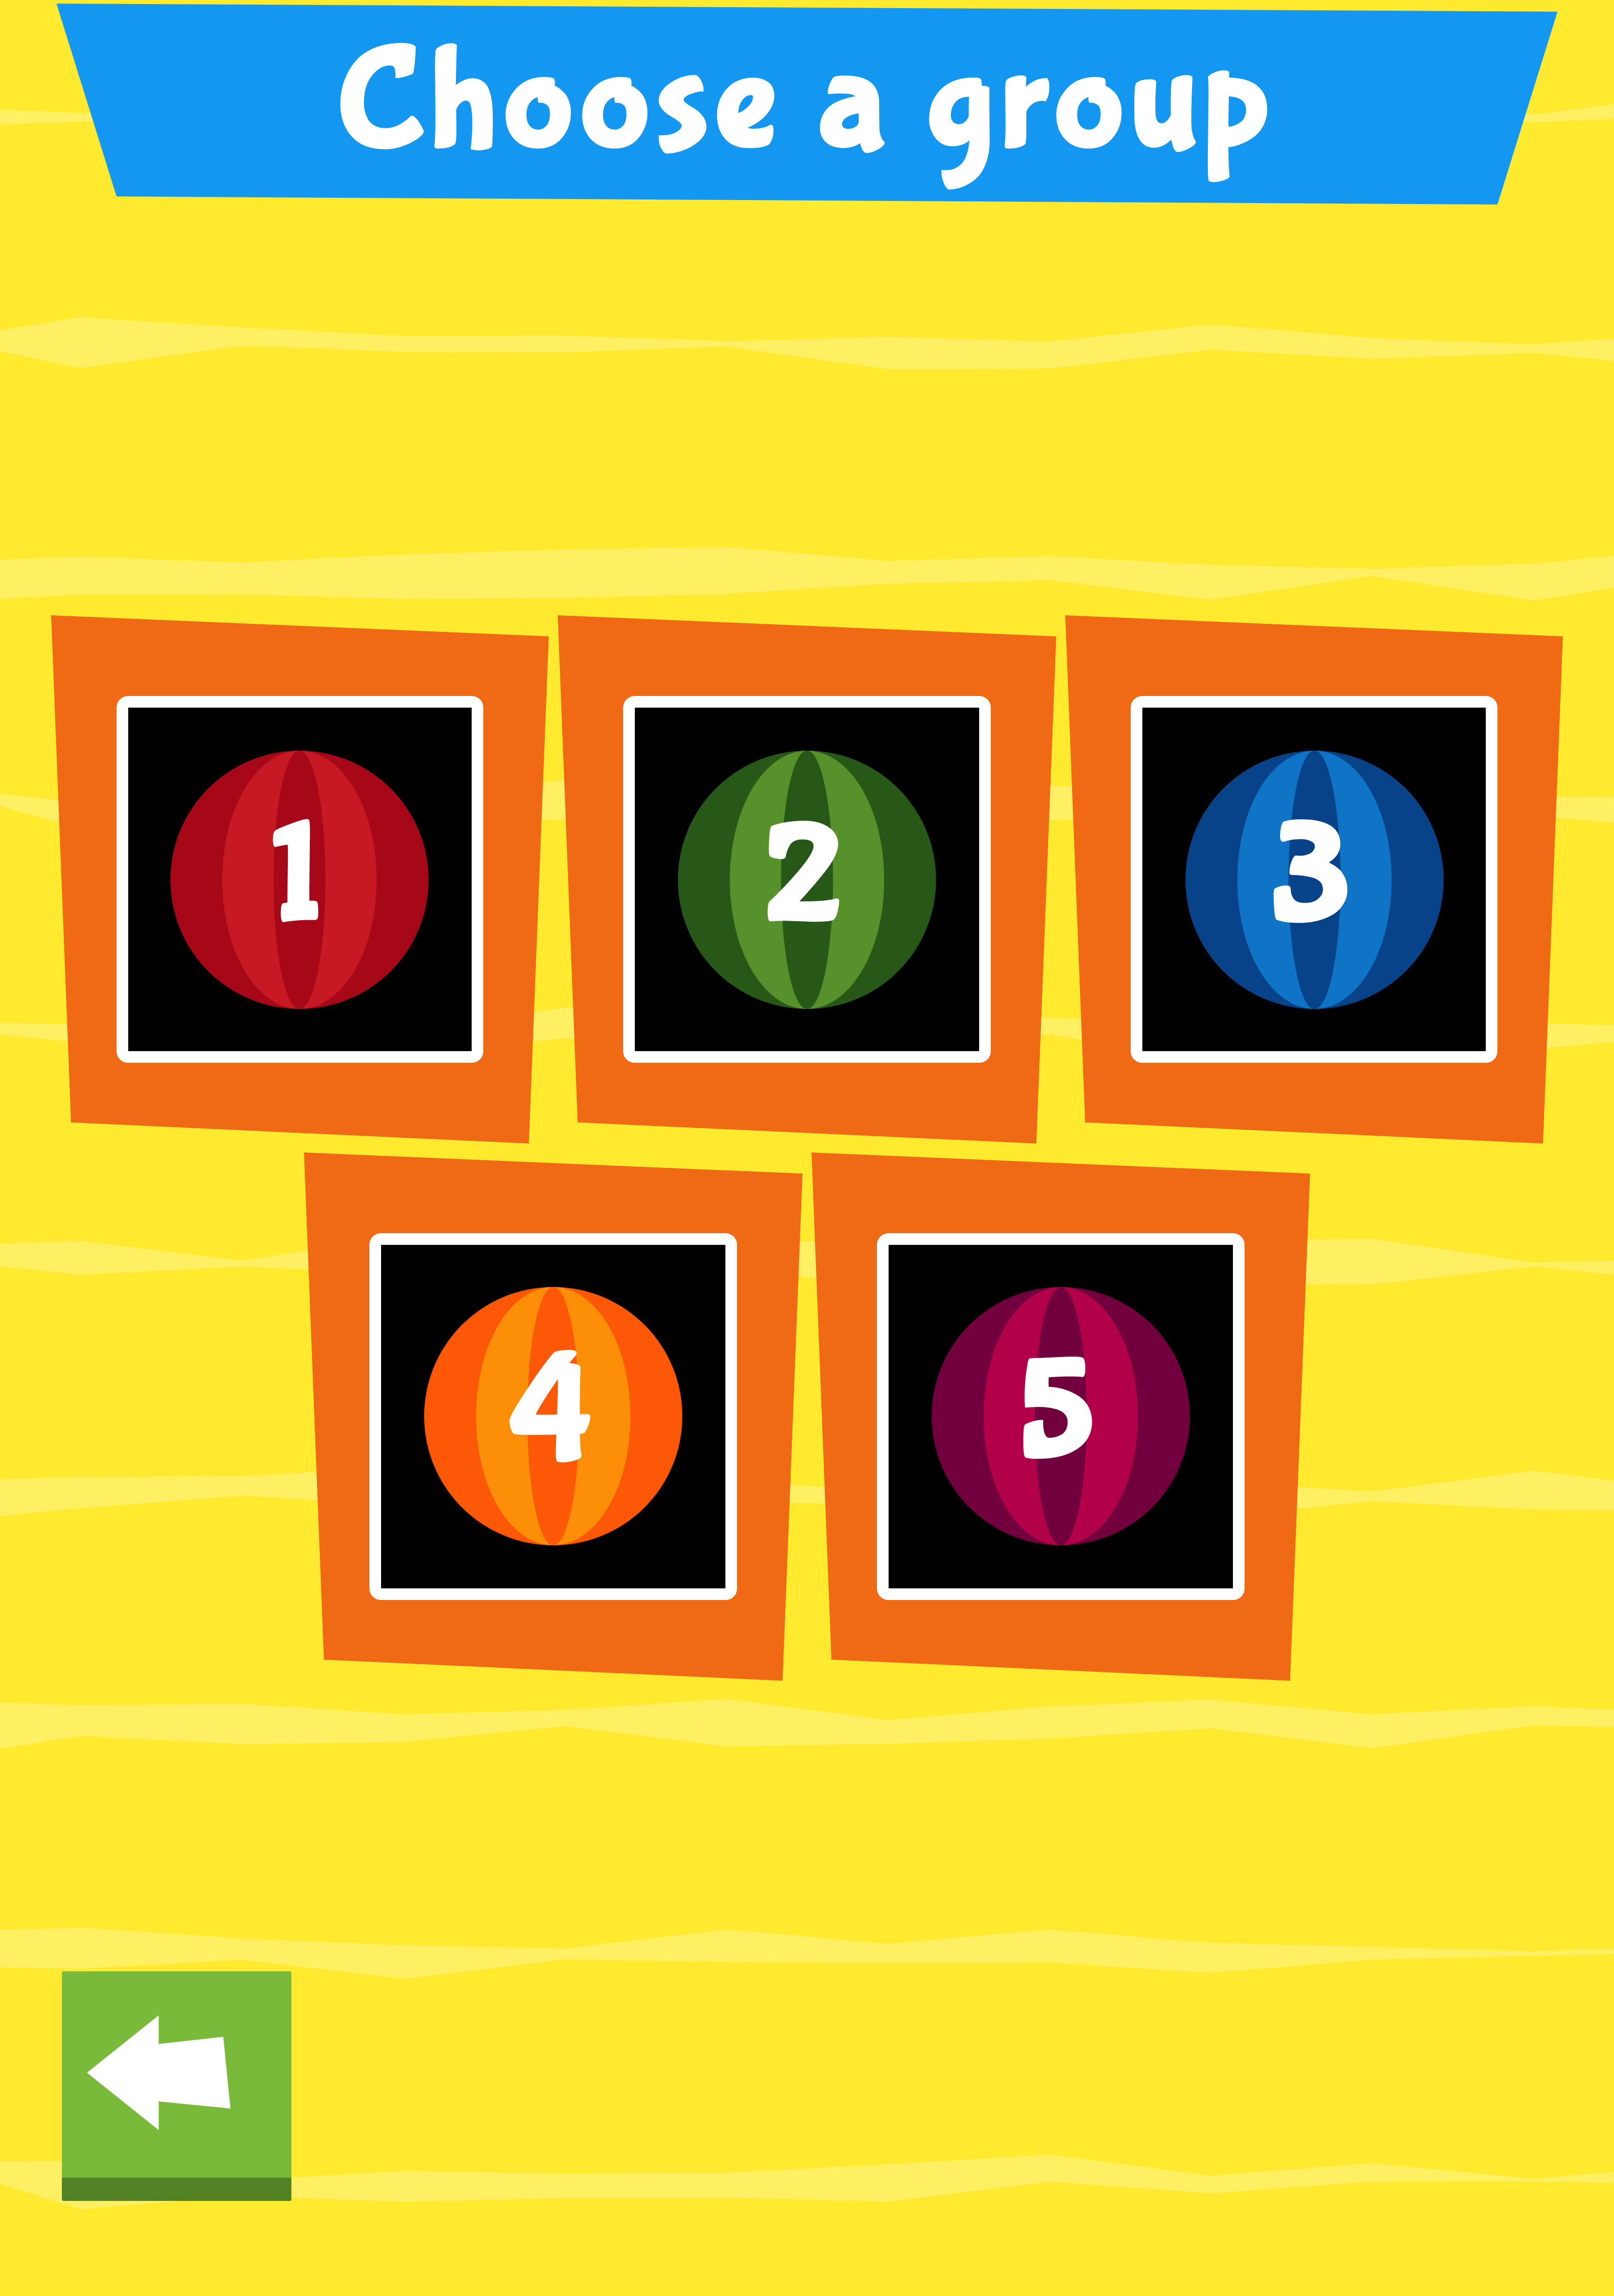
\includegraphics[width=\linewidth]{images/CALVin-screenshots/jpgs/choose_group}
  \end{column}
  \begin{column}{\screenshotwidth}
    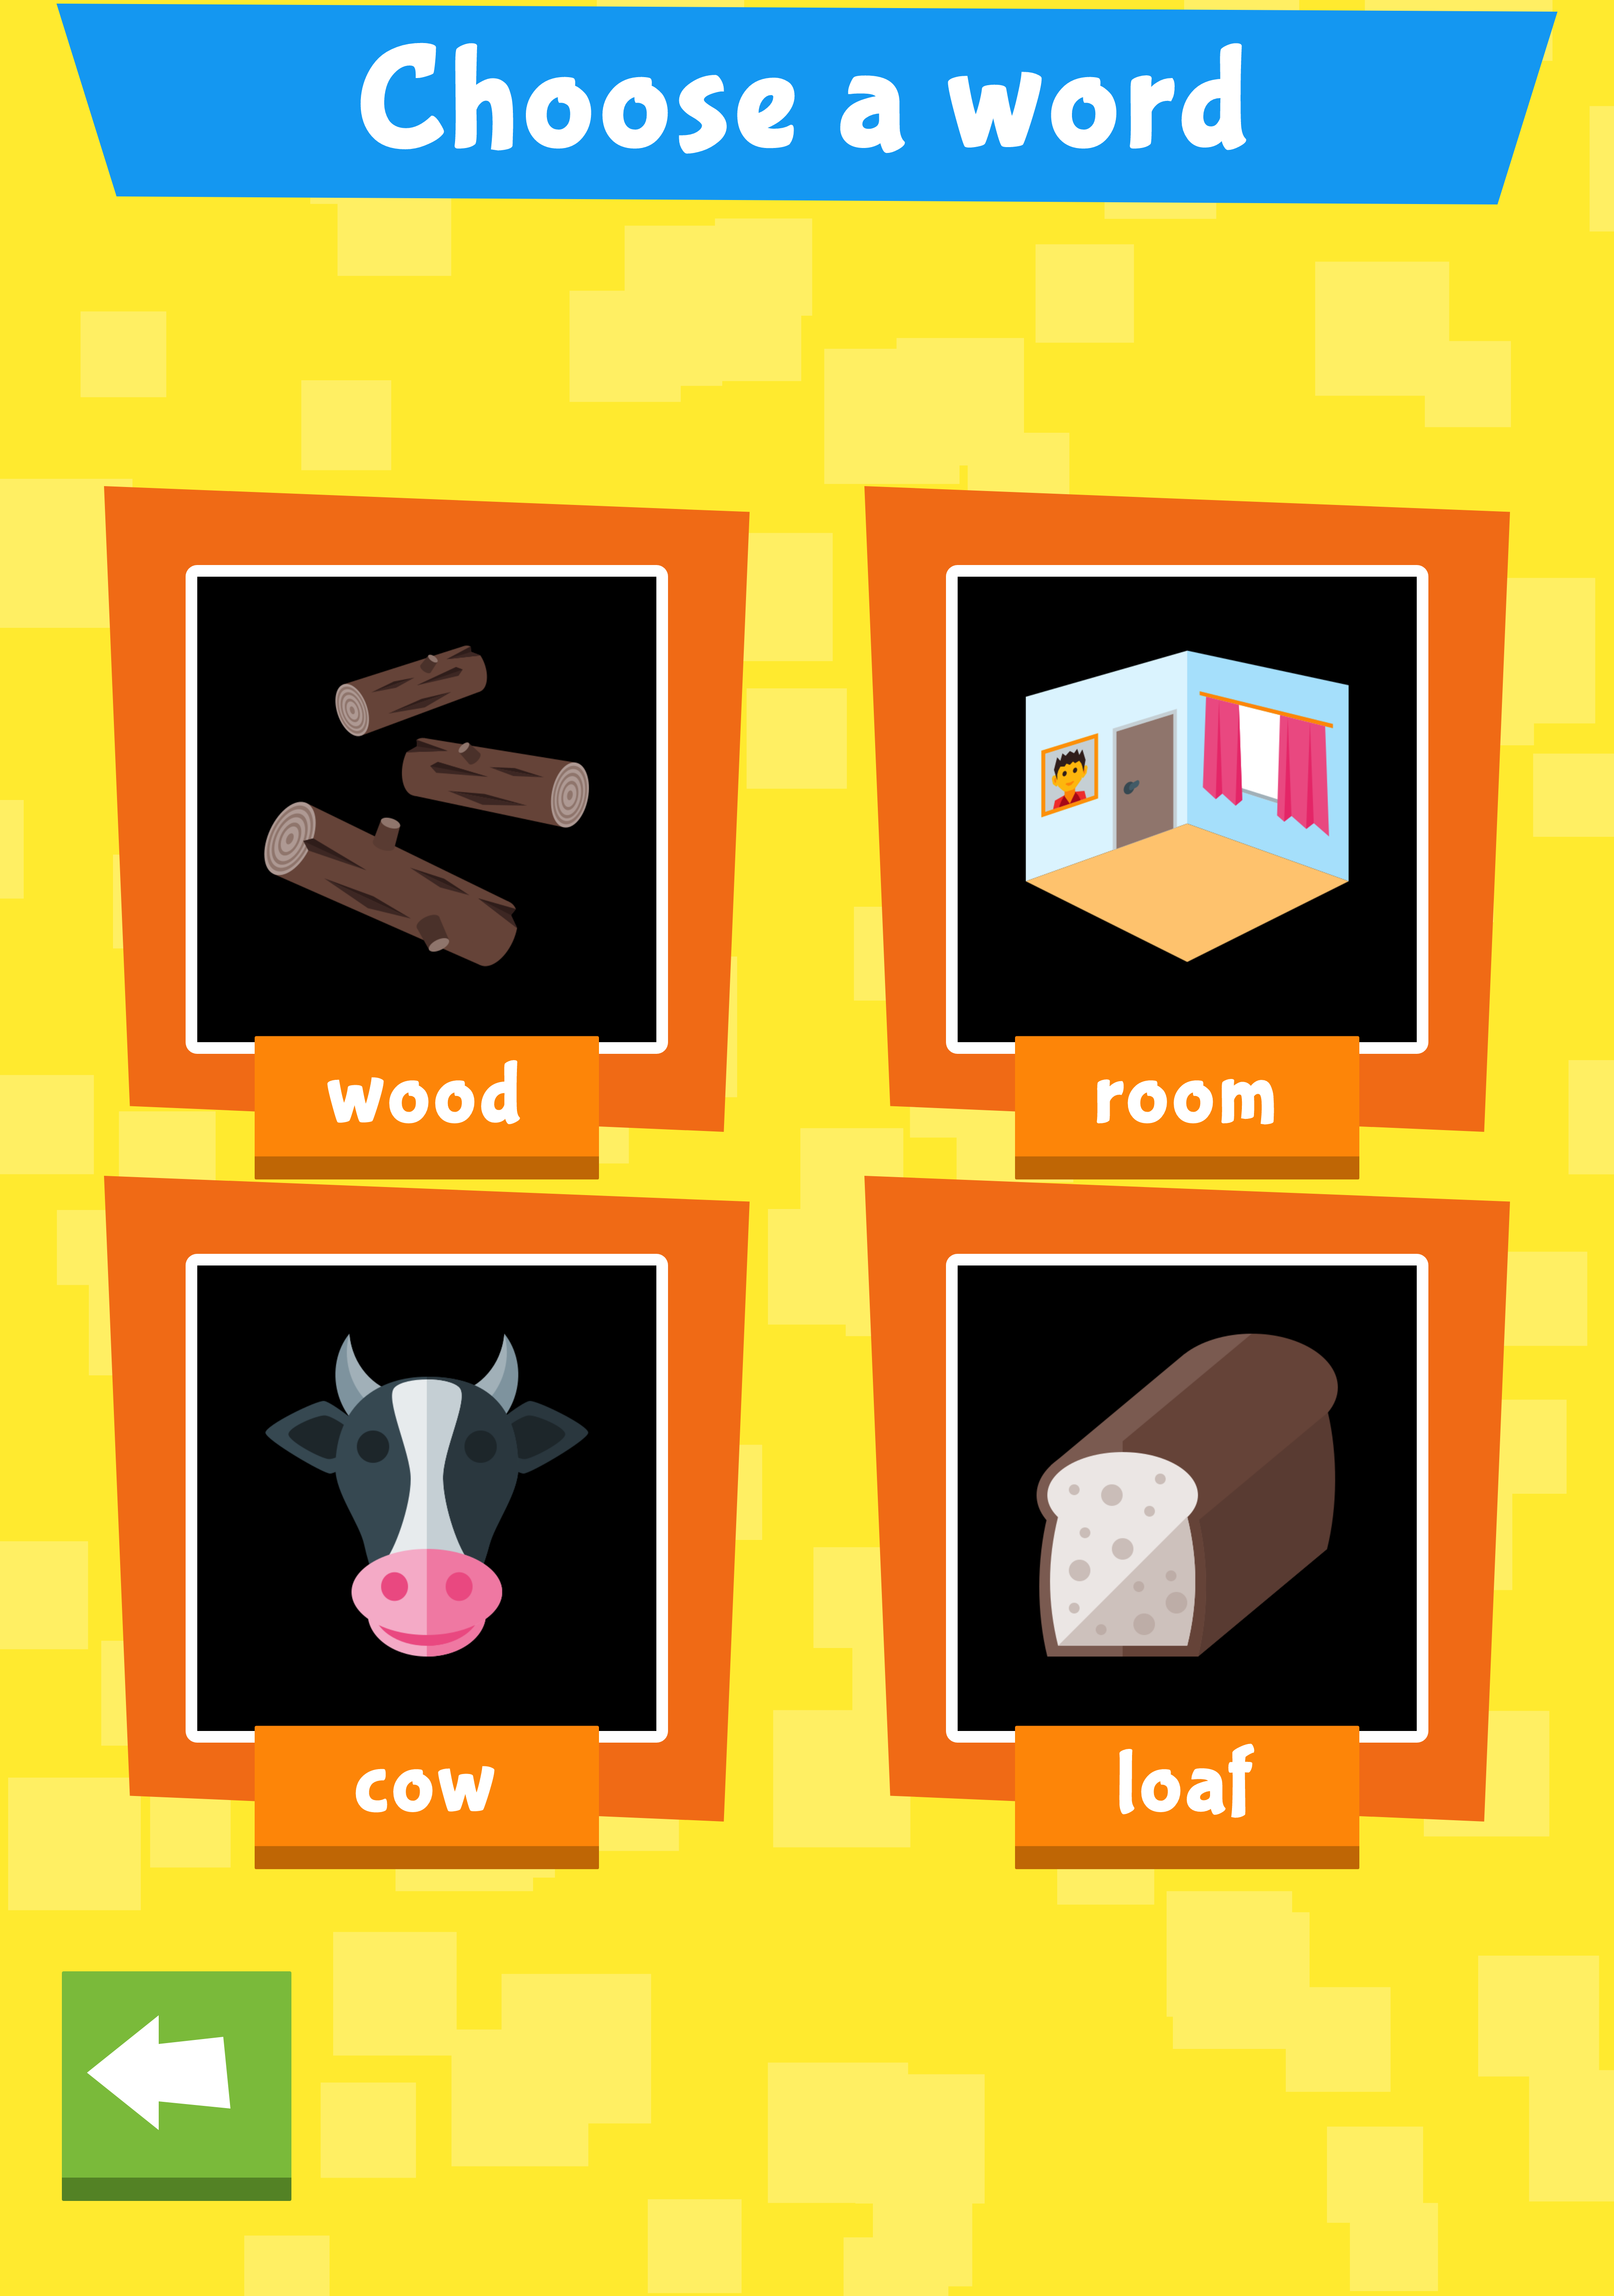
\includegraphics[width=\linewidth]{images/CALVin-screenshots/jpgs/choose_word}
  \end{column}
\end{columns}
\vspace*{1ex}
\begin{columns}
  \begin{column}{\screenshotwidth}
    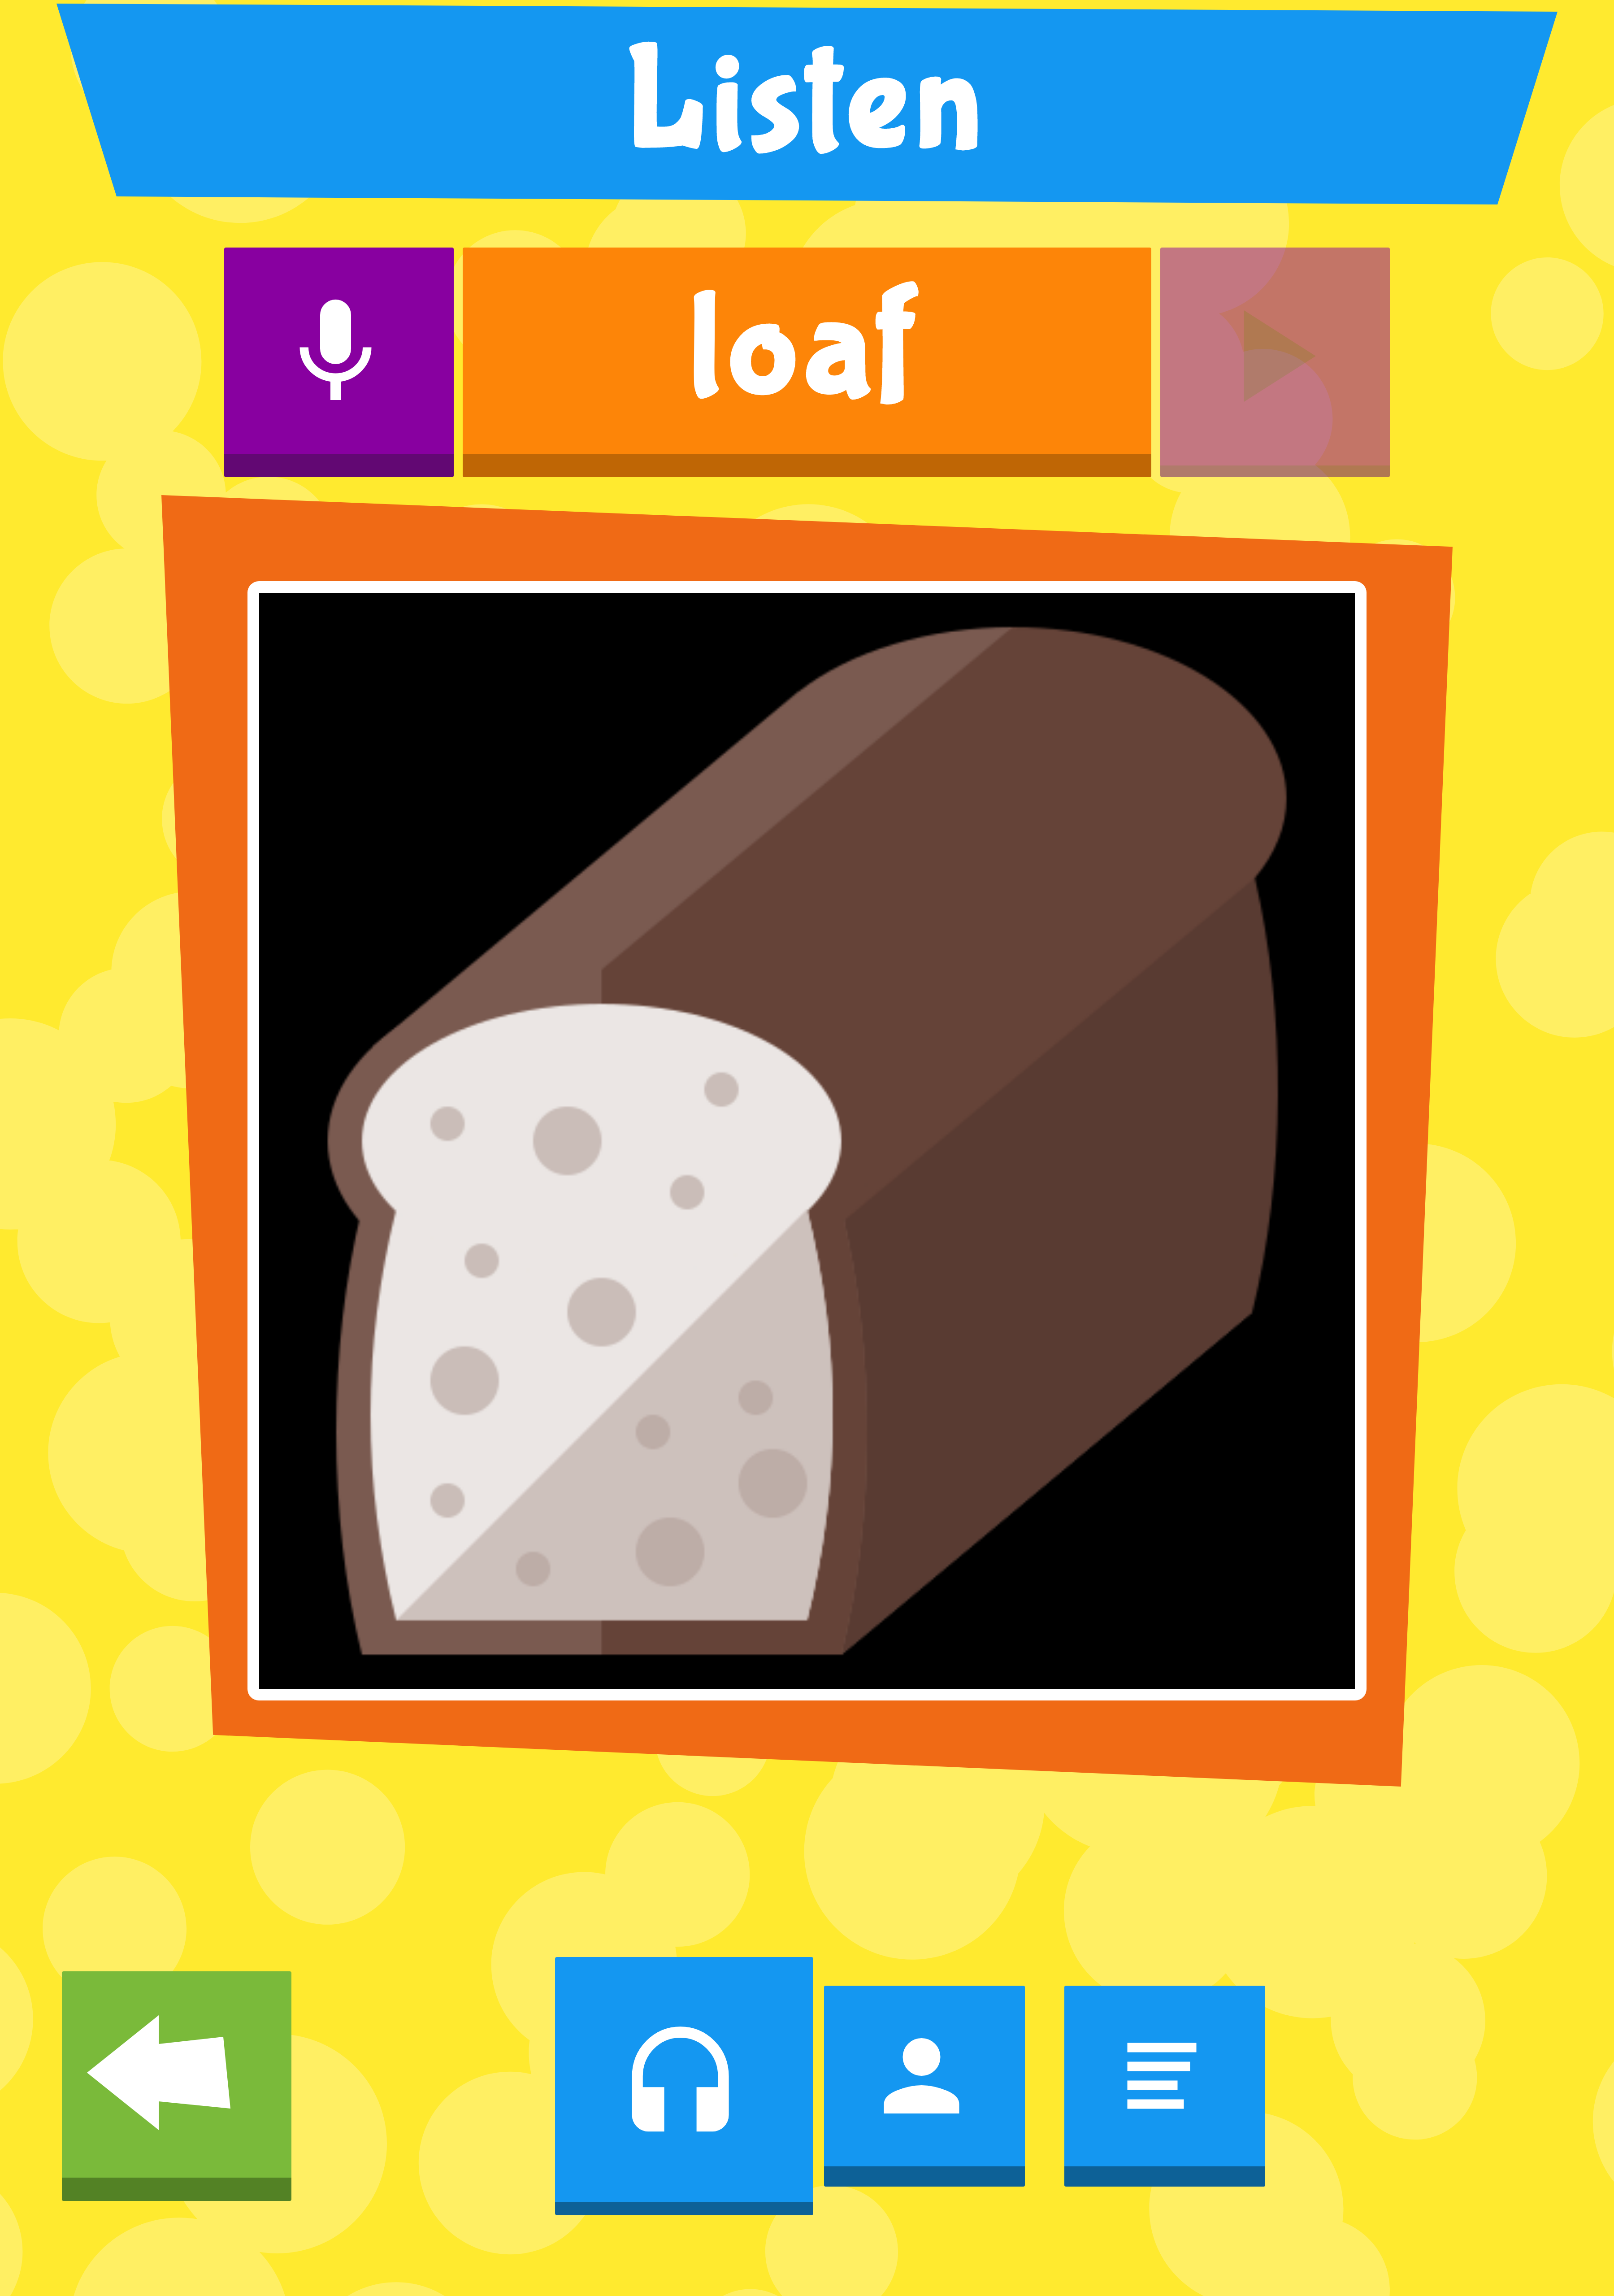
\includegraphics[width=\linewidth]{images/CALVin-screenshots/jpgs/word}
  \end{column}
  \begin{column}{\screenshotwidth}
    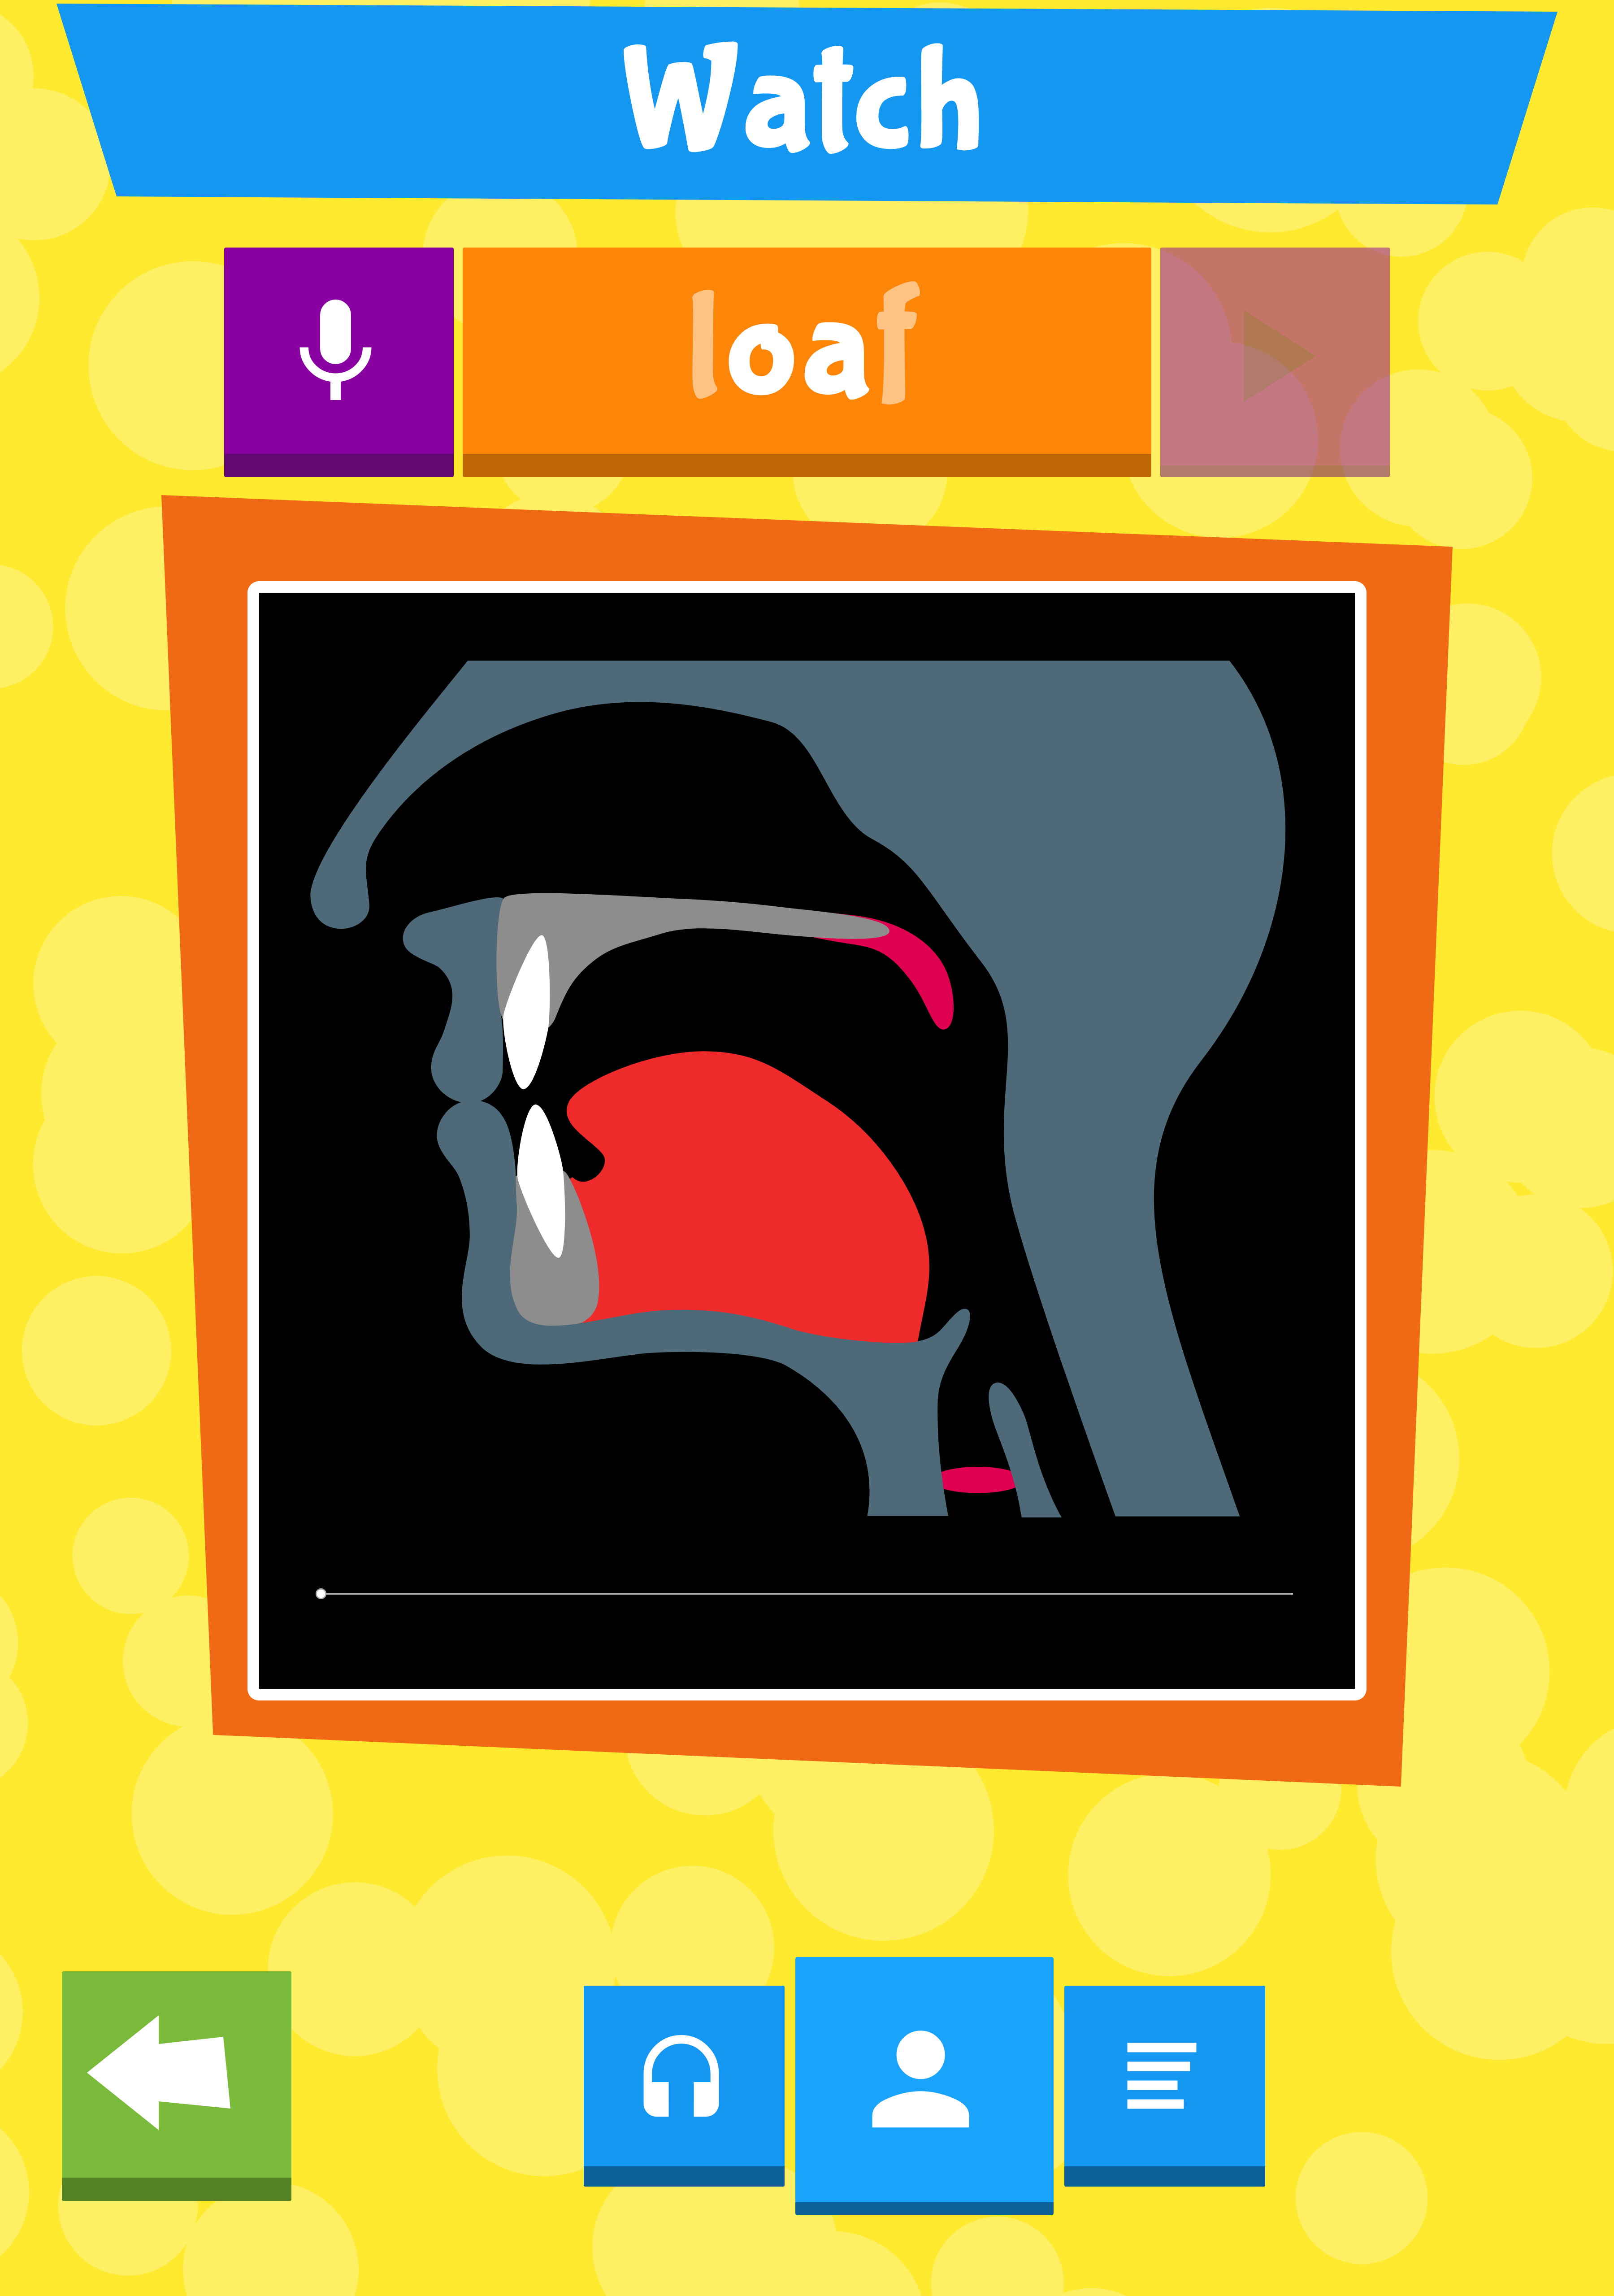
\includegraphics[width=\linewidth]{images/CALVin-screenshots/jpgs/vocal_tract_animation}
  \end{column}
  \begin{column}{\screenshotwidth}
    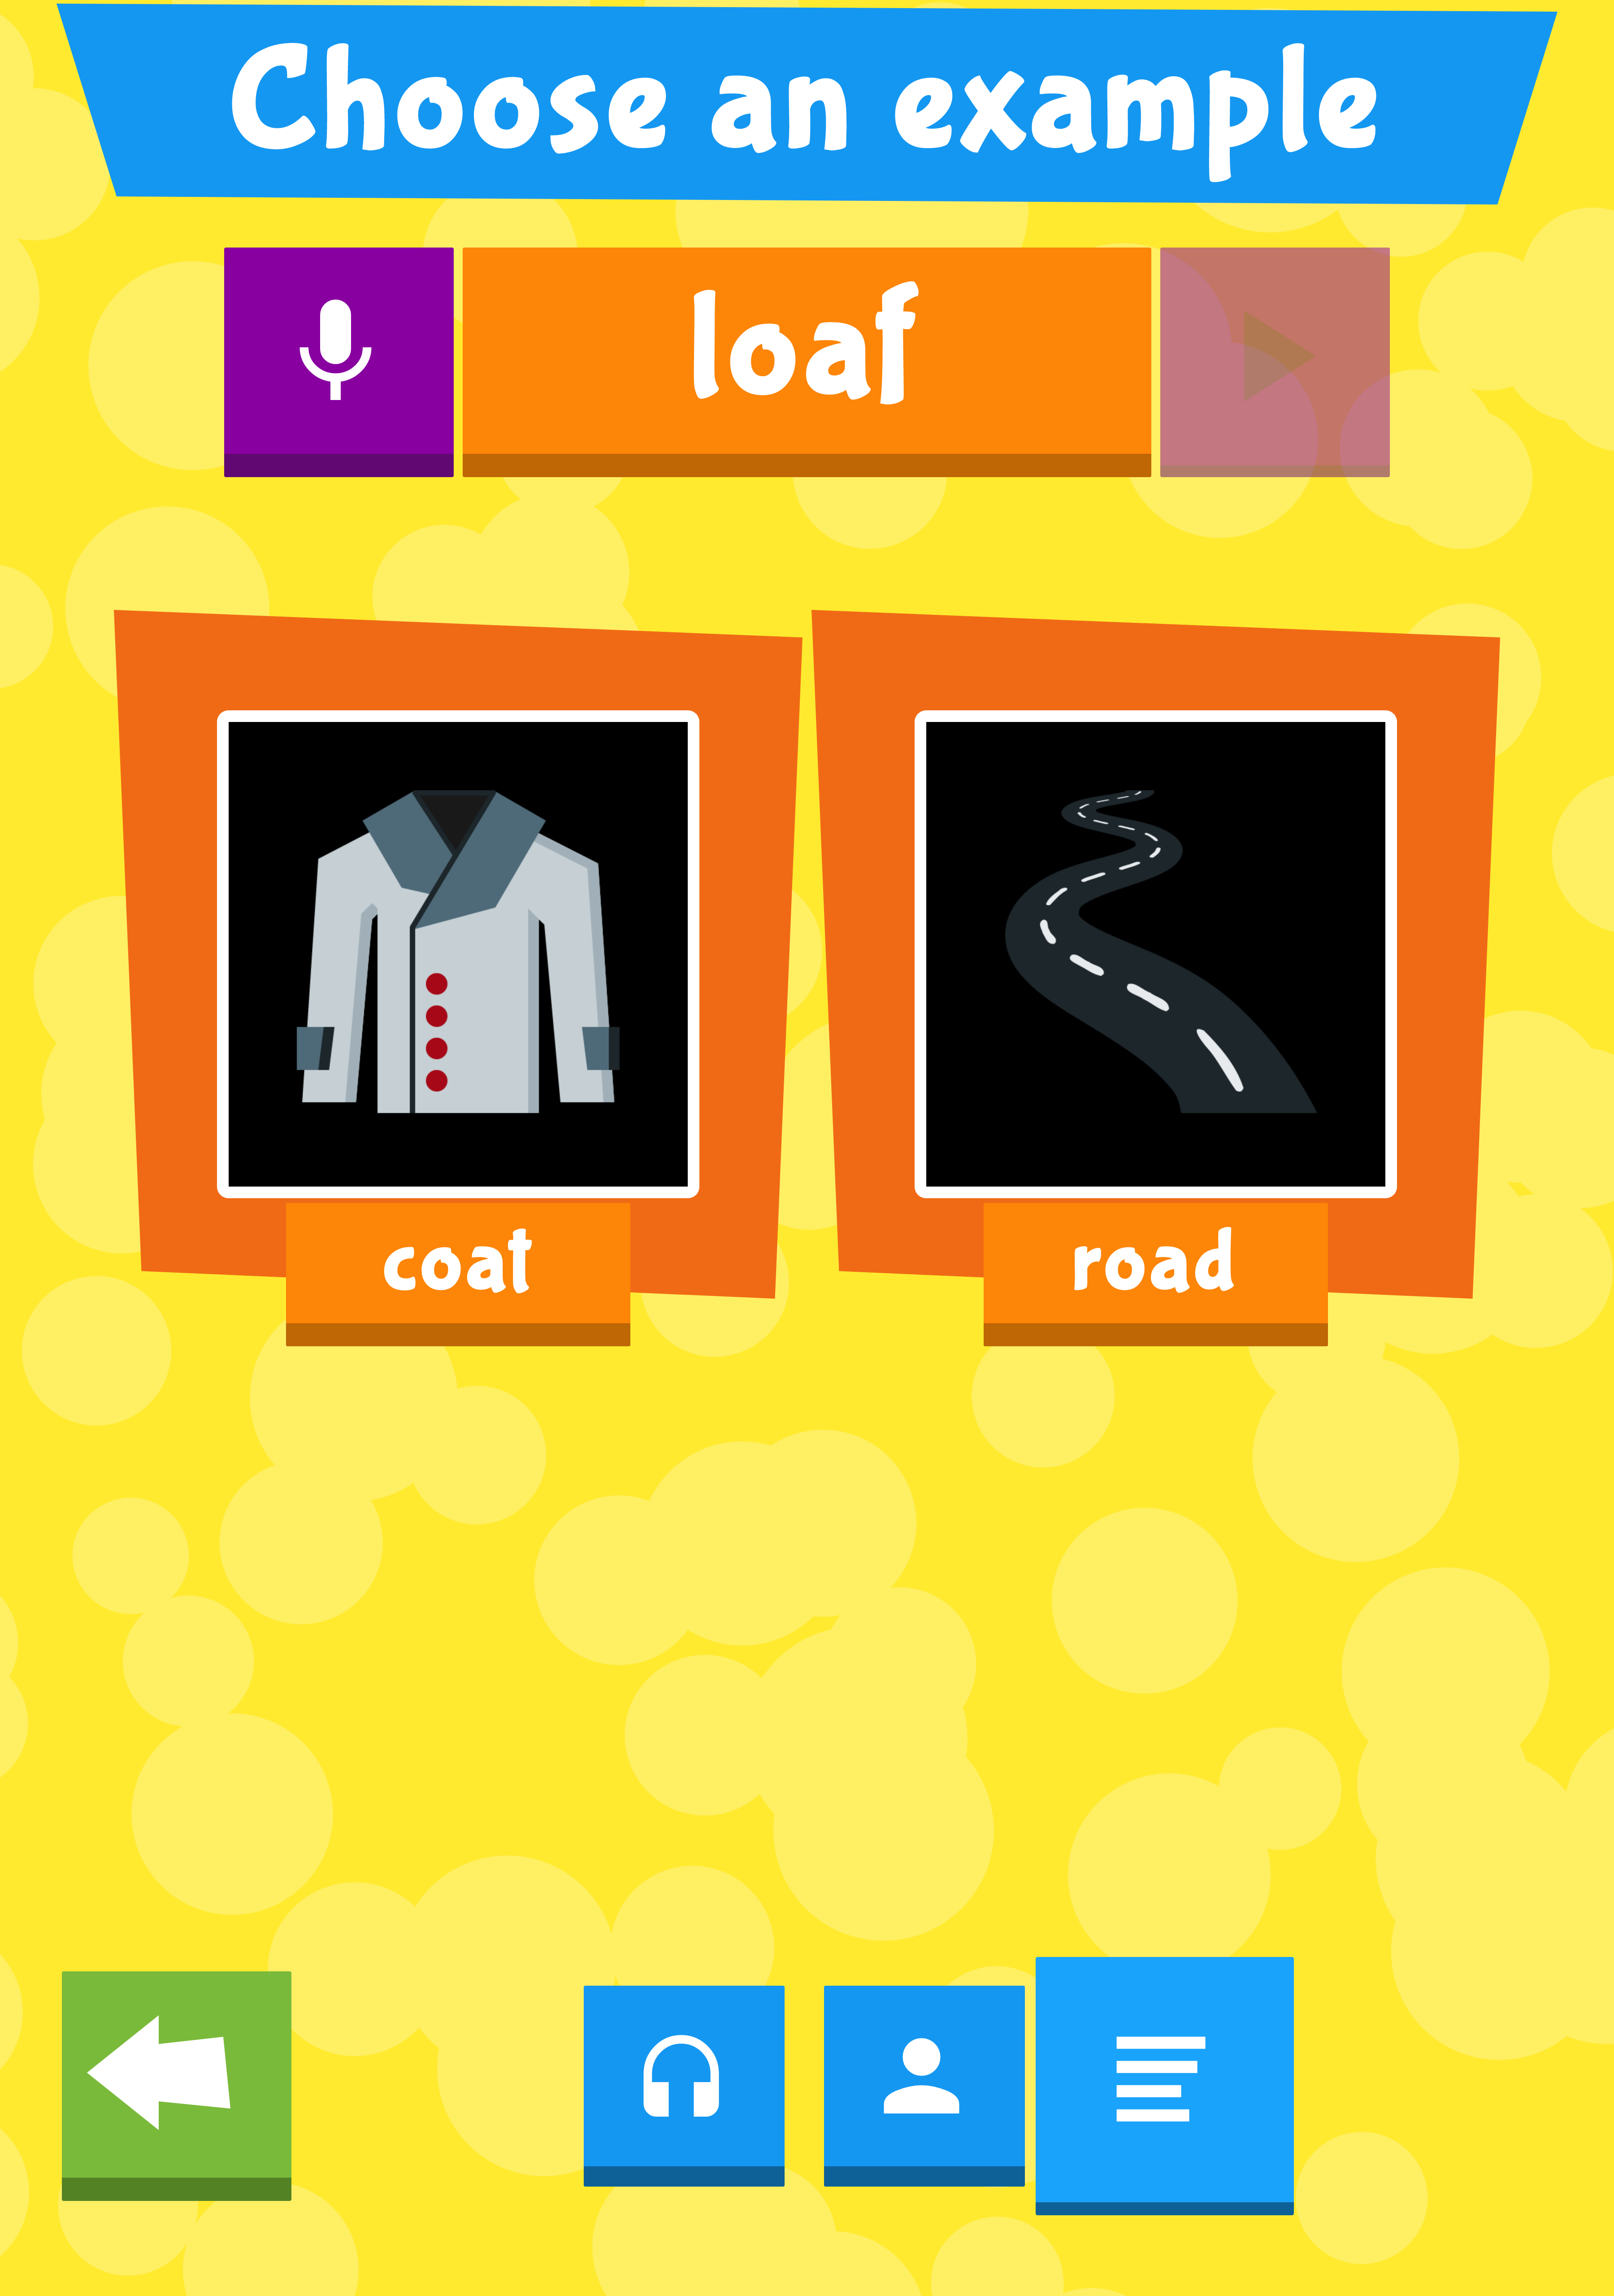
\includegraphics[width=\linewidth]{images/CALVin-screenshots/jpgs/choose_example}
  \end{column}
  \begin{column}{\screenshotwidth}
    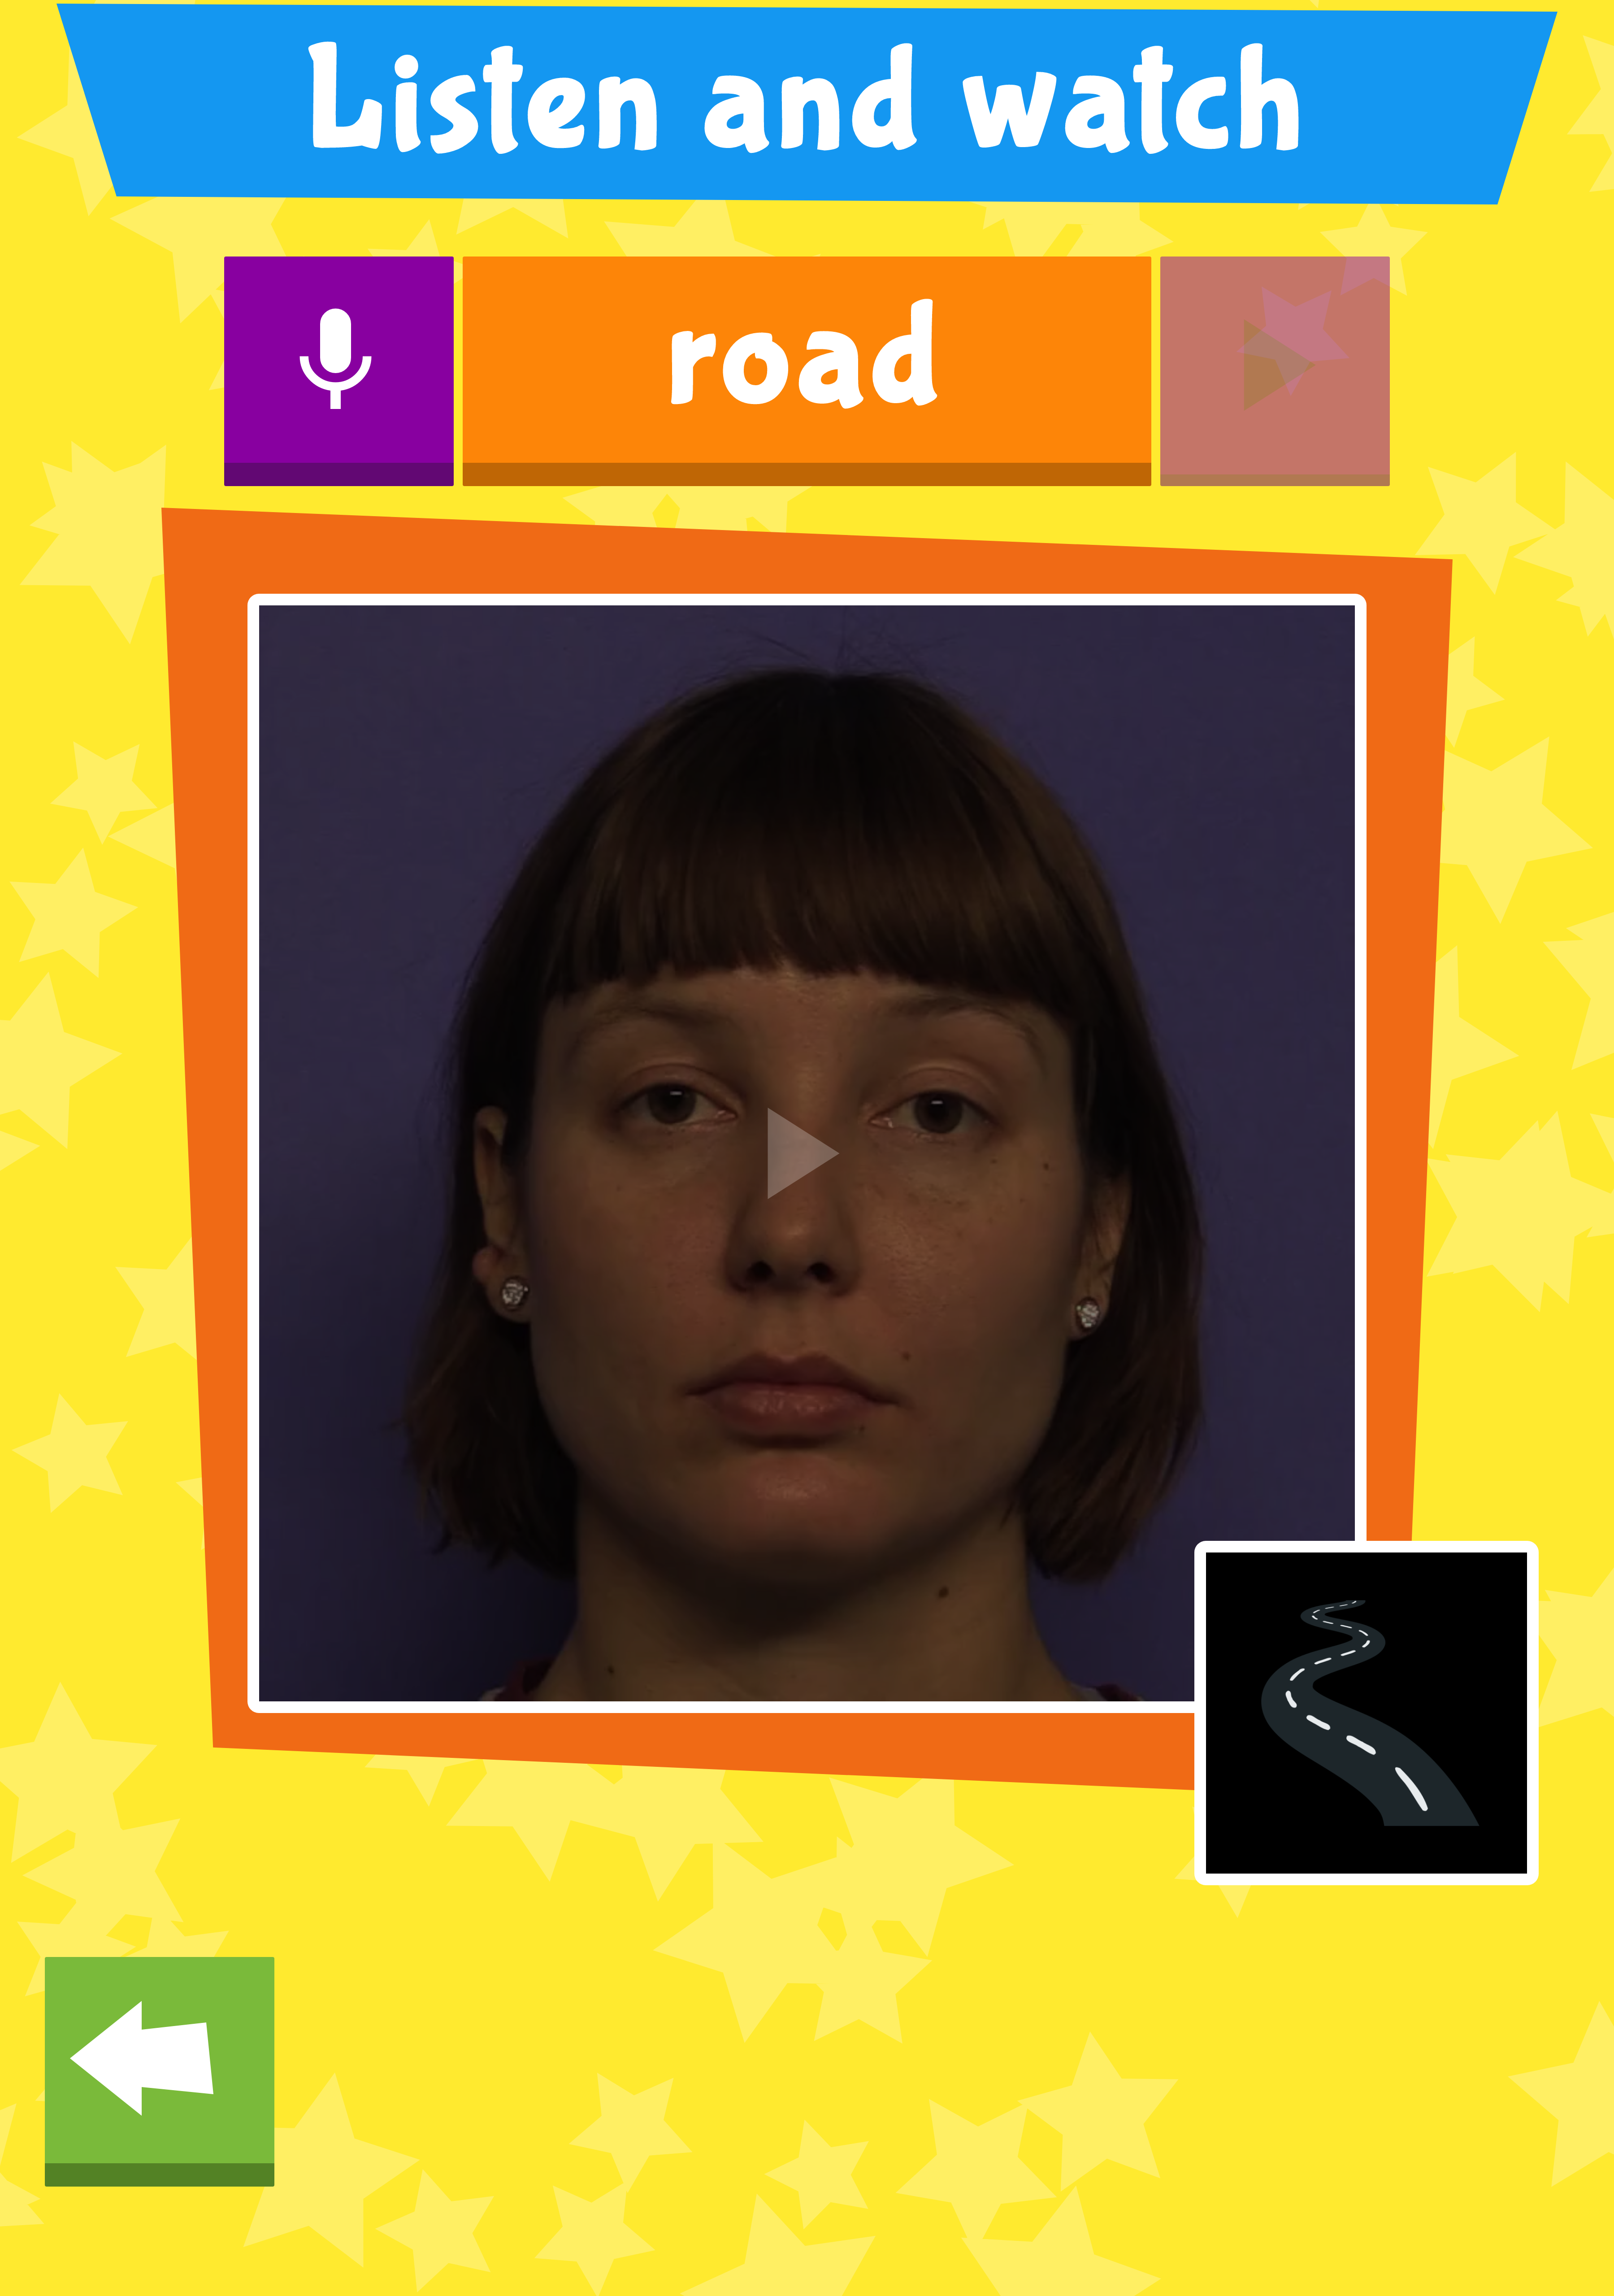
\includegraphics[width=\linewidth]{images/CALVin-screenshots/jpgs/watch_example}
  \end{column}
\end{columns}
\setbox0=\vbox{\caption{}}
\end{figure}
\vspace*{0.25in}
% \begin{itemize}
%   \item Provides audio, video and images for carrier words
%   \item Shows an animated vocal tract for individual vowels
%   \item Enables participants to record and practice vowel production
% \end{itemize}
\end{block}

\end{column}
\begin{column}{0.525\linewidth}
\begin{block}{Results}
\vspace*{0.125in}
\begin{figure}[h]
  \begin{minipage}{.45\textwidth}
\begin{tikzfigure}[oddity-boxplot]
\includegraphics[width=\linewidth]{plots/images/oddity-boxplot.png}
\end{tikzfigure}
\end{minipage}\hskip0.05\textwidth%
\begin{minipage}{.45\textwidth}
  \begin{tikzfigure}[vid-boxplot]
  \includegraphics[width=\linewidth]{plots/images/vid-boxplot.png}
  \end{tikzfigure}
\end{minipage}
\end{figure}
%
\vspace*{-0.25in}
%
\begin{figure}[h]
\begin{tikzfigure}[vowel-plot]
\includegraphics[width=0.95\linewidth]{plots/images/vowel-plot.png}
\end{tikzfigure}
\end{figure}
%
%



\paragraph{Perception (category discrimination)}

\begin{itemize}
\item
A linear mixed-effects logistic regression model showed a significant effect of training:
\hbox{\chisq (1) = 9.122}, \hbox{p < .05} --- see figure \tikzfigureref{oddity-boxplot}
\item
No significant difference between training groups, but a significant
interaction between training group and test:
\hbox{\chisq (1) = 4.667}, \hbox{p < .05}
\item
LV group performed slightly better at post-test than the HV group:
\hbox{b = -0.1998}, \hbox{SE = 0.0924}, \hbox{z = 2.161}, \hbox{p < .05}
\end{itemize}


\paragraph{Production (vowel intelligibility)}

\begin{itemize}
  \item
    Significant change in vowel production accuracy from pre- to post-test,
    \hbox{\chisq (1) = 16.762}, \hbox{p < .001} --- see figure \tikzfigureref{vid-boxplot}
  \item
    Significant effect of training group,
    \hbox{\chisq(1) = 7.65}, \hbox{p < .01}
  \item
    Planned contrasts showed that the LV group performed slightly better than the HV group,
    \hbox{b = 0.374}, \hbox{SE = 0.141}, \hbox{z = 2.645}, \hbox{p < .01}
\end{itemize}



\paragraph{Production (imitation task)}

\def\op{\hskip0.2ex}
\begin{itemize}
\item Both LV and HV children show some changes in vowel production
between pre-tests and post-tests.
Vowels centres --- SSBE vowels from \citep{hawkins_midgely_2005} ---
shown in figure \tikzfigureref{vowel-plot}
\item
Linear mixed models showed no significant change in F1 or F2 from pre- to post-test

% \item
%  Monophthong duration
%  increases significantly between pre-tests and post-tests
%  for both LV and HV groups [\op F\textsubscript{1, 723}\op=\op68.532, p\op<\op0.001\op]
%  --- see figure \tikzfigureref{duration-plot}

\end{itemize}


\end{block}


\begin{block}{Conclusions}

\begin{itemize}
  \item
    Children improved in both their vowel perception and production (albeit subtly)
  \item
    LV training group showed slightly better performance after only 5 training sessions
  \item
    LV seems to be more beneficial for children in learning new articulatory targets \cite{evans_martin-alverez_2016}
  \item
    Inspection of the acoustic analysis suggests that children were able to generalize
    their learning in production to new stimuli in the imitation task
    (F2 values approached native-like realizations for some vowels:
    \ipa{/ɜː/}, \ipa{/ɑː/}, \ipa{/ʊ/})%, \ipa{/eə/}, \ipa{/ɪə/})

  \item
    Future research may focus on smaller subsets of vowels and  one-to-one training
\end{itemize}
\end{block}

\vspace*{-0.125in}

\begin{block}{\small References}
  \renewcommand\bibfont{\tiny}
  \printbibliography
\end{block}

%\vspace*{-0.125in}

\textbf{Acknowledgements}

  This work was supported by
  grant G-474-270-38 from King Abdulaziz University

\end{column}

\end{columns}

\end{frame}

\end{document}
